\documentclass[a4paper,10pt]{article}
\usepackage[utf8]{inputenc}
\usepackage{amssymb}
\usepackage{graphicx}
\usepackage{graphics}
\usepackage{listings}
\usepackage{color}
\definecolor{dkgreen}{rgb}{0,0.6,0}
\definecolor{gray}{rgb}{0.5,0.5,0.5}
\definecolor{mauve}{rgb}{0.58,0,0.82}
\renewcommand{\familydefault}{\rmdefault}

\lstset{ %
  language=C++,                % the language of the code
  backgroundcolor=\color{white},      % choose the background color. You must add \usepackage{color}
  showspaces=false,               % show spaces adding particular underscores
  showstringspaces=false,         % underline spaces within strings
  showtabs=false,                 % show tabs within strings adding particular underscores
  keywordstyle=\color{dkgreen},          % keyword style
  commentstyle=\color{blue},       % comment style
  stringstyle=\color{red},         % string literal style
  }

\begin{document}
\thispagestyle{empty}
Using the solver:
\begin{lstlisting}
#include "finite_difference.h"

using namespace std;

int main() {

	int n = 100;
	int m = 100;

	Grid first_grid;
	first_grid.load_grid(n,m);
	first_grid.set_flow(100, -100);
	first_grid.set_halfcircle_east(50,50,20,0);

	Finite_Difference fd;
	fd.to_solve(first_grid);
	fd.set_precision(0);
	fd.solve();
	Grid sol = fd.get_solution();
	//cout << fd.number_of_iterations() << endl;
	sol.gnuplot_values();
	

	return 0;

	}\end{lstlisting}
	
\newpage

Creating your own boundary functions:
\begin{lstlisting}
void set_circle(int x, int y, unsigned int r, double val) {
	if(x - r < 0 || x + r > values.size() - 1 || y - r < 0 || 
	y + r > values[0].size() - 1)cout << "Out of range." << endl;
	else {
		for (int xs = x-r; xs<=x+r; xs++) {
			for(int ys = y-r; ys<=y+r; ys++) {
			Coordinate xy;
			xy.set_xy(xs,ys);
			Coordinate mid;
			mid.set_xy(x,y);
			if( mid.distance(xy) < r )
			{values[xs][ys].value = val; 
			values[xs][ys].boundary = true;}
			}
		}
	}
}
\end{lstlisting}
\newpage
Plotting in gnuplot:



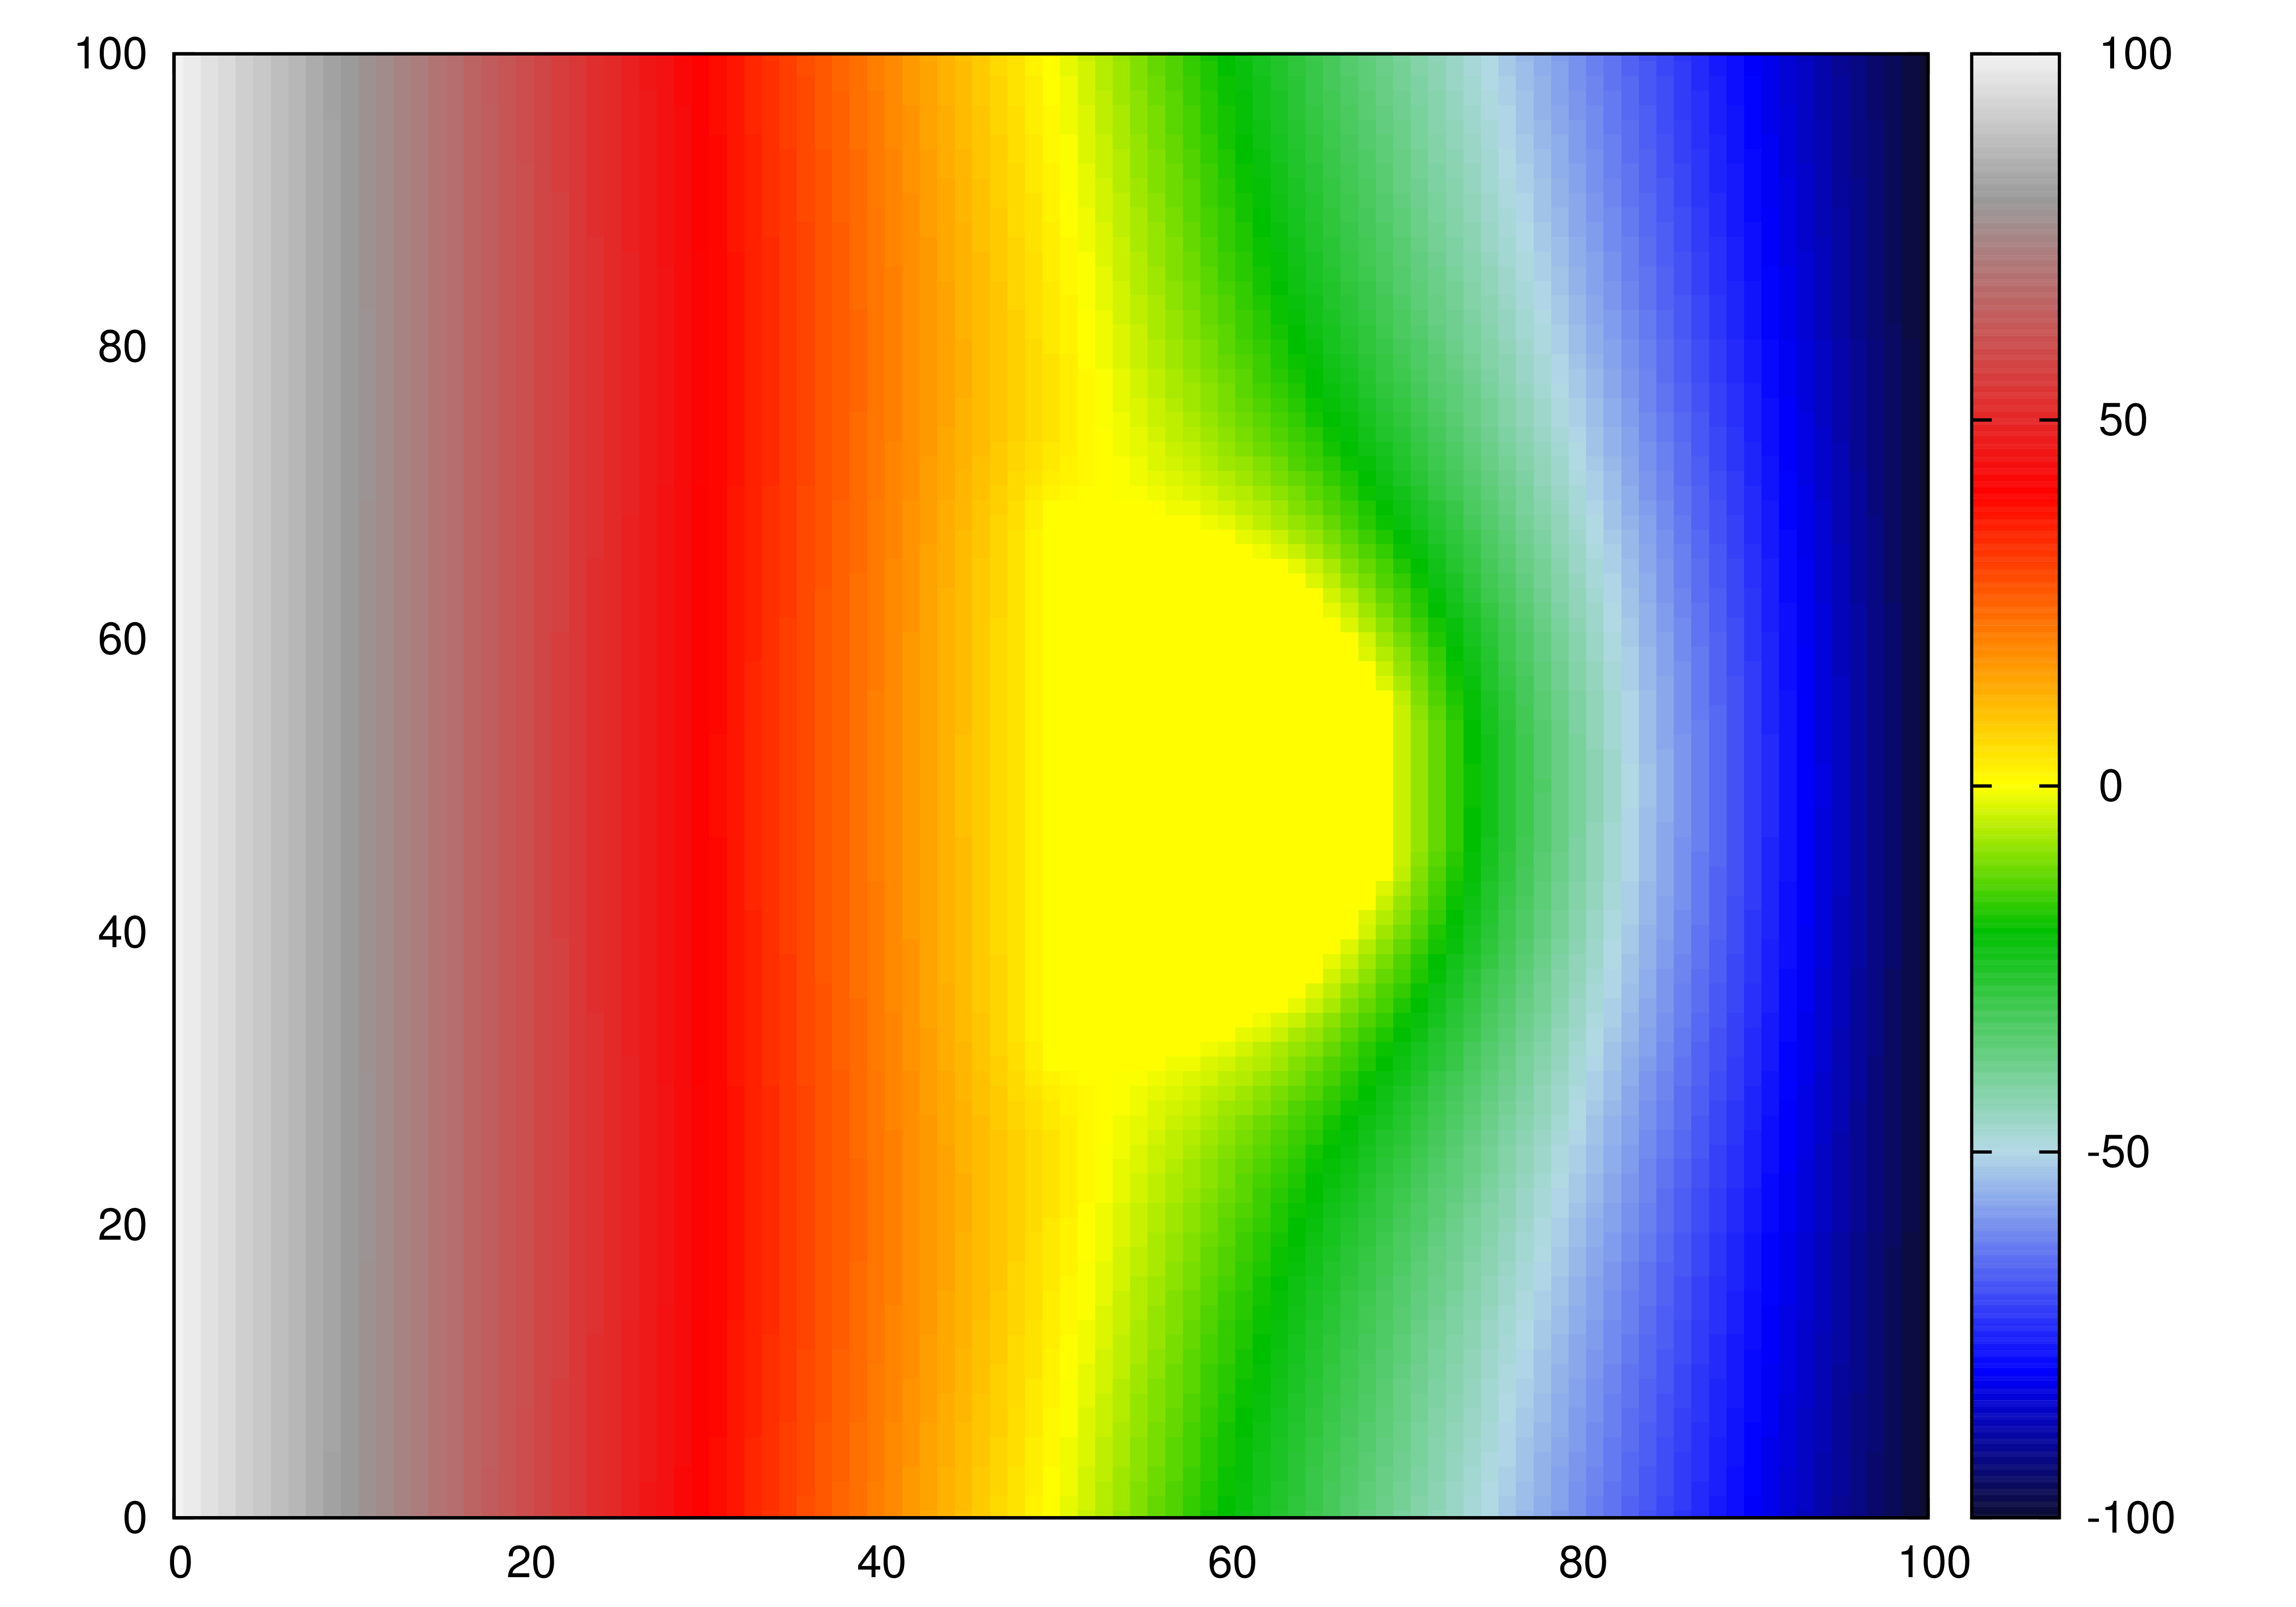
\includegraphics[width=\textwidth]{circle.png}



Use $grid.gnuplot\_values()$ and don't print anything else in your program.
\vspace{1cm}

Redirect output to data file ( $./my\_program > data.dat$ )
\vspace{1cm}

gnuplot $>$ plot 'data.dat' matrix with image


\vspace{3cm}


Various options possible, example file on github.


\end{document}